
%% see http://latex-beamer.sourceforge.net/
%% idea contributed by H. Turgut Uyar
%% template based on a template by Till Tantau
%% this template is still evolving - it might differ in future releases!

\documentclass[xcolor={usenames,dvipsnames}]{beamer}
\usepackage{booktabs}


% THEME
% =========================================================
%\usetheme{Boadilla}
\setbeamertemplate{navigation symbols}{}
\setbeamercolor{normal text}{fg=white,bg=black!90}
\setbeamercolor{structure}{fg=white}
\setbeamercolor{item projected}{use=item,fg=white,bg=item.fg!35}
\setbeamercolor*{palette primary}{use=structure,fg=structure.fg}
\setbeamercolor*{palette secondary}{use=structure,fg=structure.fg!95!black}
\setbeamercolor*{palette tertiary}{use=structure,fg=structure.fg!90!black}
\setbeamercolor*{palette quaternary}{use=structure,fg=structure.fg!95!black,bg=black!80}
\setbeamercolor*{framesubtitle}{fg=white}
\setbeamercolor*{block title}{parent=structure,bg=black!60}
\setbeamercolor*{block body}{fg=black,bg=black!10}
\setbeamercolor*{block title alerted}{parent=alerted text,bg=black!15}
\setbeamercolor*{block title example}{parent=example text,bg=black!15}
%\useinnertheme[shadow]{rounded}
% =========================================================

% DEFINE COLORS
% =========================================================
\definecolor{darkred}{RGB}{223,63,00}
\definecolor{brightred}{RGB}{255,127,00}
% =========================================================

% Templates
% =========================================================
%\setbeamertemplate{itemize subitem}[triangle]
% =========================================================

% SET COLORS
% =========================================================
\setbeamercolor{normal text}{fg=white,bg=black!90}
\setbeamercolor{structure}{fg=white}
\setbeamercolor{item projected}{use=item,fg=white,bg=item.fg!35}
\setbeamercolor*{palette primary}{use=structure,fg=structure.fg}
\setbeamercolor*{palette secondary}{use=structure,fg=structure.fg!95!black}
\setbeamercolor*{palette tertiary}{use=structure,fg=structure.fg!90!black}
\setbeamercolor*{palette quaternary}{use=structure,fg=structure.fg!95!black,bg=black!80}
\setbeamercolor*{framesubtitle}{fg=white}
\setbeamercolor*{block title}{parent=structure,bg=black!60}
\setbeamercolor*{block body}{fg=black,bg=black!10}
\setbeamercolor*{block title alerted}{parent=alerted text,bg=black!15}
\setbeamercolor*{block title example}{parent=example text,bg=black!15}
% =========================================================


% FONTS
% =========================================================
\setbeamerfont{alerted text}{series=\bfseries}
% =========================================================


% PACKAGES
% =========================================================
\usepackage[english]{babel}
\usepackage[utf8]{inputenc}
\usepackage{DejaVuSansMono}
\usepackage[T1]{fontenc}
\usepackage{tikz}
% =========================================================

% METADATA
% =========================================================
\title{Formal Methods in IT Security --- WS 2022/23}

\subtitle{Seminar}

\author[M. Tschirschnitz]
{
	Maximilian von Tschirschnitz
}

\institute[Chair I20, TUM]
{
	Lehrstuhl f\"ur Sicherheit in der Informatik / I20 \\
	Prof.\ Dr.\ Claudia Eckert\\
	Technische Universität München
}

\date{\today}
% =========================================================

\begin{document}

\begin{frame}
	\titlepage
\end{frame}

\begin{frame}
	\frametitle{A Presentation on Presentations}

	\hfill
	\begin{itemize}
		\item Presenting a paper \emph{relates to} writing a paper.
		\item \alert{as}
		\item Playing theater \emph{relates to} writing a book.
	\end{itemize}
\end{frame}

%
\begin{frame}[label=process]
	\frametitle{YOU are the storyteller}
	\begin{itemize}
		\item Use your arms and legs.
		\item Use your face.
		\item Use your voice.
		\item Talk with passion to excite others.
	\end{itemize}
\end{frame}

\begin{frame}[label=process]
	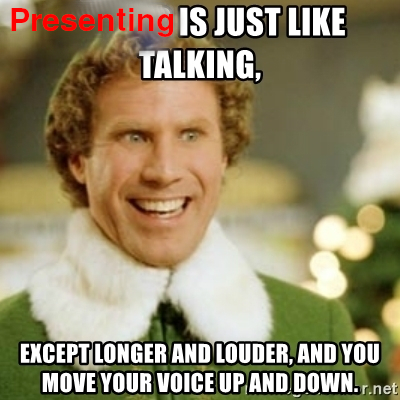
\includegraphics[height=\paperheight]{presenting.jpg}
\end{frame}

\begin{frame}[label=process]
	\begin{itemize}
		\item Get others excited for your topic!
		\item Face your audience
		\item Move!
	\end{itemize}
\end{frame}

\begin{frame}
	\frametitle{Visuals and slides}
	They are only here to \alert{support}.
	\begin{enumerate}
		\item \alert{No more} then 5 pieces of information on a slide.
		\item Main information through the `visual and audial track' (you)
		\item Use graphics (oversized arrows and boxes are ok!).
		\item Your slides do not have to work standalone.
	\end{enumerate}
\end{frame}

\begin{frame}
	\frametitle{Content}
	\begin{enumerate}
		\item Your presentation is \alert{not} the audiobook of your paper.
		\item Not every element has to re-occur $\rightarrow$ reduce to essentials.
		\item Tell us what you did, reasoned.
		\item Maintain a flow.
	\end{enumerate}
\end{frame}

\begin{frame}
	\begin{enumerate}
		\item Focus on the motivation behind your topic.
		\item Related Work and Background only if required for your presentation.
		\item Avoid deep reasoning \alert{but} be ready to answer deep questions. 
		\item Demo / Discussion ?
	\end{enumerate}
\end{frame}

\begin{frame}
	\frametitle{Practice, Practice, Practice}
	\begin{enumerate}
		\item Talk yourself through multiple times (I know it sucks).
		\item Time yourself!
		\item Check your flow.
		\item Relax your body and voice; move!
	\end{enumerate}
\end{frame}

\begin{frame}
	\frametitle{Format}
	\begin{enumerate}
		\item Presentations should take $\approx$ 30 minutes.
		\item 15 minutes of questions.
		\item Your responsibility to have everything ready and tested.
		\item Reminder: Paper and slides are due on the last day of the Semester.
	\end{enumerate}
\end{frame}




\begin{frame}
	\begin{center}
		{\huge Questions?}

	\end{center}
\end{frame}


\end{document}
